Now, the next step is to compute a valid set of data using odometry and gyro data. By the nature of the data type, odometry data is accurate for robot moving in a linear motion, but is inaccurate when the robot is turning due to wheel slippage. In contrast, gyro data is a good resource for estimating the turning angle, but performs poorly in linear motion. Thus, two optimization methods are given to combine odometry and gyro data.

One method labelled ``gyro-only" method in Figure \ref{fig:Gyrodometry} is to take odometry data as the prediction of the distance, whereas the FOG information \(\dot{\psi}_{\text{IMU}}\) is used for predicting the heading of the robot. 

One other optimization is the ``gyrodometry" method discribed in section.\ref{sec:gyrodo}. Besides, by experiment, the threshold value is set where \(C_{\dot{\psi}} = 0.2\)

\begin{figure}
    \centering
    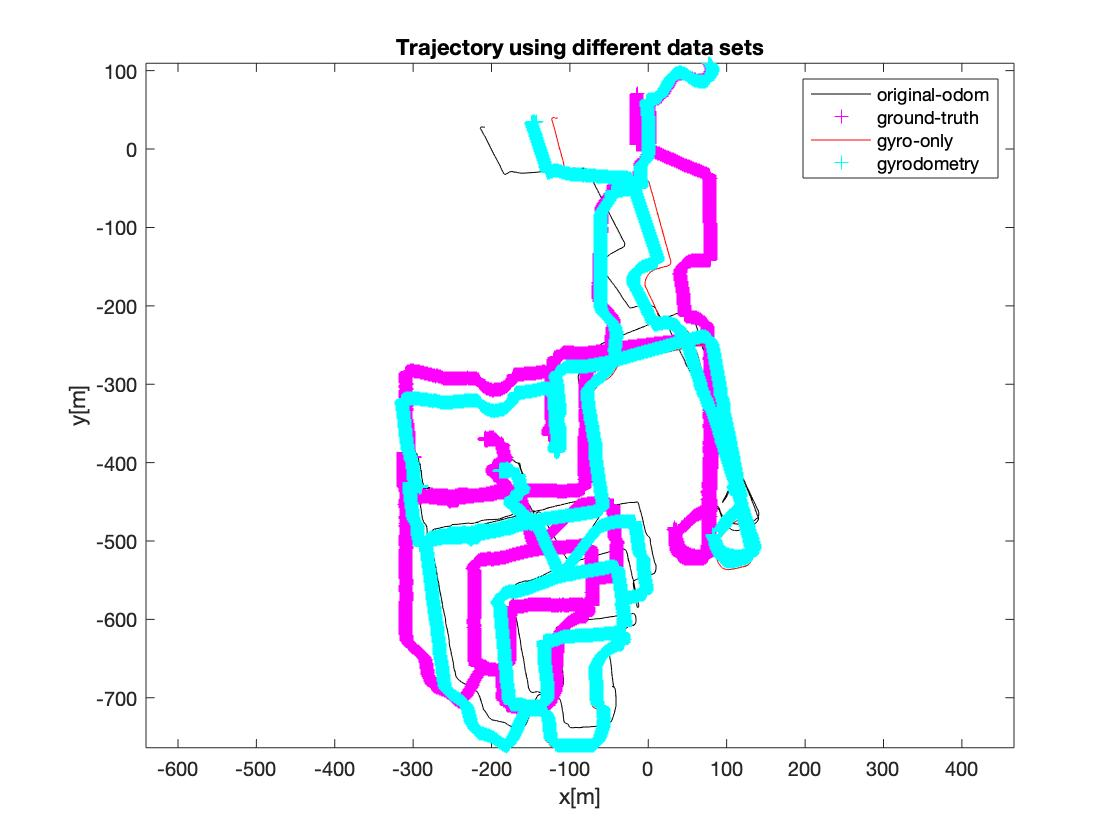
\includegraphics[width=0.8\columnwidth]{media/Gyrodometry.jpg}
    \caption{Odometry optimization using Gyrodometry method}
    \label{fig:Gyrodometry}
\end{figure}